\chapter{Special Discrete Random Variables}
\begin{definition}{}{}
  A discrete random variable \(X\) which takes all values in \(\mathbb{Z}^{+}_{0}\) is a \emph{binomial distribution} with probability of success \(p\), denoted by \(X \sim \operatorname{B}(n,p)\), iff
  \[\Prob(X=x)=\binom{n}{x}p^x(1-p)^{n-x}.\]
\end{definition}
\begin{definition}{}{}
  A discrete random variable \(X\) which takes all values in \(\mathbb{Z}^{+}\) has a \emph{geometric distribution} with probability of success \(p\), denoted by \(X \sim \operatorname{Geo}(p)\), iff
  \[\Prob(X=x)=(1-p)^{x-1}p.\]
\end{definition}
\begin{note}
  We can assume \(X \sim \operatorname{B}(n,p)\) (or \(W \sim \operatorname{Geo}(n,p)\)) iff the following three conditions hold
  \begin{enumerate}
    \item The event of a [trial in context] is independent of that of another [trial in context].
    \item The probability of each [trial in context] is constant.
    \item Each trial has only two mutually exclusive outcomes.
  \end{enumerate}
\end{note}
\begin{note}
  Defining random variables:
  \begin{enumerate}
    \item Binomial distribution: Let \(X\) be the number of [trial in context], out of [number of trials \(n\) in context]. 
    \item Geometric distribution: Let \(W\) be the number of [trial in context], up to and including the first [successful trial in context].
  \end{enumerate}
\end{note}
\begin{note}
  Let \(W \sim \operatorname{Geo}(p)\), and \(q\coloneq 1-p\). Then,
  \begin{enumerate}
    \item \(\Prob(W>m)=q^m\),
    \item \(\Prob(X>m+n \,\vert\, X>n)=\Prob(X>m)=q^m\),\item \(\Prob(X<m+n \,\vert\, X>n)=\Prob(X<m)=1-q^{m-1}\).
  \end{enumerate}
  (The last two represent the memorylessness of the geometric distribution.)
\end{note}
\begin{definition}{}{}
  A discrete random variable \(X\) which takes all values in \(\mathbb{Z}_{0}^{+}\) has a \emph{Poisson Distribution} with parameter \(\lambda>0\), denoted by \(X \sim \operatorname{Po}(\lambda)\), iff 
  \[\Prob(X=x)=\frac{e^{-\lambda}\lambda^x}{x!}.\]
\end{definition}
\begin{note}
  We can assume \(Y \sim \operatorname{Po}(\lambda)\) iff the following three conditions hold
  \begin{enumerate}
    \item The event of a [trial in context] is \emph{independent} of that of another [trial in context].
    \item The \emph{mean number of occurrences} of [trial in context] is \emph{constant} over an fixed interval of time/space.
    \item The \emph{mean number of occurrences} of [trial in context] is \emph{proportional} to the length of the space/time interval.
    % 
    % The banished.
    % 
    % \item The \emph{probability} of [trial in context] occurring at \emph{any point} in space/time within a small fixed interval of space/time is \emph{the same}.
    % \item The \emph{probability} of \emph{more than one} occurrence in any infinitesimally small interval is \emph{negligible}.  
  \end{enumerate}
\end{note}
\begin{note}
  Additive property of the Poisson distribution: If \(U \sim \operatorname{Po}(\mu)\) and \(V \sim \operatorname{Po}(\lambda)\) are \emph{independent} variables, then 
  \[U+V \sim \operatorname{Po}(\mu+\lambda).\]
\end{note}
\begin{note}
  Defining random variables: Let \(Y\) be the number of [event in context], in [space/time interval in context].  
\end{note}
\begin{note}
  Explain why it might be inappropriate to model \(X\) using a Poison distribution.
  \begin{center}
    \parbox{0.9\textwidth}{
      \[\widebar{x}=\rule{0.5cm}{0.01mm} \qquad\qquad s^2=\rule{0.5cm}{0.01mm}\]
      If \(X\sim\Poisson(\lambda)\) is an appropriate model for some \(\lambda\), then the population mean and population variance of \(X\) should coincide. But this may not be true, because the sample mean differs significantly from the unbiased estimate for sample variance. Hence, a Poisson distribution may be an inappropriate model for \(X\).
    }
  \end{center}
\end{note}
\begin{example}{Validity of a Poisson model.}{}
  Let \(\mathscr{X}\) be a discrete random variable and consider the approximation/model \(X\sim\Poisson(\lambda)\). Suppose that \(\Prob(\mathscr{X}=m)\approx\Prob(X=n)\) and \(\Prob(\mathscr{X}=n)\approx\Prob(X=n)\) for some integers \(m\) and \(n\).  Comment on whether this information validates the use of the Poisson model?
  \begin{center}
    \parbox{0.9\textwidth}{
      No: two specific outcomes are not enough to validate the use of the Poisson model. Instead, we need to consider all possible outcomes.
    }
  \end{center}
\end{example}
\begin{stbox}{General Information}
  \begin{enumerate}
    \item Expectation and Mean:
    \begin{center}
      \begin{tabular}{|Sc|Sc|Sc|}
        \hline
        Distribution & Expectation & Variance\\
        \hline
        \(X \sim \operatorname{B}(n,p)\) & \(np\) & \(np(1-p)\)\\
        \hline
        \(Y \sim \operatorname{Po}(\lambda)\) & \multicolumn{2}{Sc|}{\(\lambda\)}\\
        \hline
        \(W \sim \operatorname{Geo}(p)\) & \(p^{-1}\) & \((1-p)p^{-2}\)\\
        \hline
      \end{tabular}
    \end{center}
    \item Use graphing or a table to deal with questions involving inequalities
    \item It is helpful to remember the following formulas for when you're asked to derive a formula for mean/mode:
    \[\sum_{r=1}^{\infty}{rx^{r-1}}=(1-x)^{-2} \qquad\text{and}\qquad \sum_{r=1}^{\infty}{r^2x^{r-1}}=\frac{1+x}{(1-x)^3}.\]
    \item Why is the probability for (b) is smaller than that for (a):
    The case of (b) is a proper subset of (a).
    \item A discrete random variable \(M\) can have other probability distributions. In such cases, defining a random variable \(W\) having a Binomial/Poisson/Geometric distribution, and then writing \(M\) as a function of \(W\) may help.

    For example, it may be that \(M=W-1\), or \(M=W_1+W_2\).
  \end{enumerate}
\end{stbox}
\begin{note}
  When the question asks for the \emph{most likely} number of [event], it is asking for the \emph{mode}.
  \end{note}
\begin{GCSkills}{}
  Finding \emph{mode} (e.g. for binomial distributions):
  \begin{enumerate}
    \item Set \(Y_1=\texttt{binompdf}(n,p,X)\).
    \item Go to table.
    \item Find the value of \(X\) for which the highest value of \(Y_1\) occurs.
  \end{enumerate}
\end{GCSkills}
\begin{GCSkills}{}
  \begin{enumerate}
    \item \texttt{2nd + Vars + `A' \(\implies\) binompdf\((n,p,x)=\Prob(X=x)\)}
    \item \texttt{2nd + Vars + `B' \(\implies\) binomcdf\((n,p,x)=\Prob(X\leq x)\)}
  \end{enumerate}
\end{GCSkills}
\begin{note}
  Let \(X\) be the random variable such that \(X \sim \operatorname{B}(n,p)\). If \(\highlight[cyan!50]{\Prob(X=n)}\) is the \emph{highest probability} that occurs, \(X=n\) is the modal value. So, we solve the two inequalities \(\highlight[cyan!50]{\Prob(X=n)}>\highlight[orange!50]{\Prob(X=n-1)}\) and \(\highlight[cyan!50]{\Prob(X=n)}>\highlight[orange!50]{\Prob(X=n+1)}\). This gives the \emph{strictest} range of values that \(p\) can take (Fig 17.1).
\end{note}
\begin{figure}[H]
  \centering
  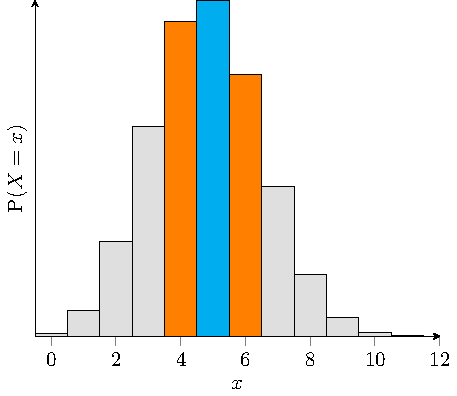
\includegraphics{../Diagrams/Binomial-Distribution/Binomial-Distribution.pdf}
  \caption{\ref{source:binomial-distribution} The histogram for a binomial distribution \(X\sim\operatorname{B}(10,p)\) that has mode \(m=5\).}
  \label{fig:binomial-distribution}
\end{figure}
\begin{example}{2018 TPJC JC2 H2 MYE P2 8}{}
  On average, 3.5\% of a certain brand of chocolate turn out misshapen. The chocolates are sold in packets of 25.
  \begin{enumerate}[label=(\roman*)]
    \item State, in context, two assumptions needed for the number of misshapen chocolates in a packet to be well modelled by a binomial distribution.
    \item Explain why one of the assumptions stated in part (i) may not hold in this context.
  \end{enumerate}
  \textit{Answer:}
  \begin{enumerate}[label=(\roman*)]
    \item 
    \begin{enumerate}[label=\arabic*.]
      \item Each chocolate is \emph{equally likely} (3.) to be misshapen.
      \item The event that a chocolate is misshapen is \emph{independent} (2.) of the event that another chocolate is misshapen.
    \end{enumerate}
    \item While on average, the probability that a chocolate is misshapen is 3.5\%, it is possible that there are more misshapen chocolates at certain times, possible due to equipment malfunction, which would mean the probability is not constant.\\[3mm]
    OR\\[3mm]
    Misshapen chocolates could be the result of equipment used and as the equipment used would not be the same for the same portion of the chocolate produced, whether a chocolate is misshapen may not be independent of another chocolate being misshapen.
  \end{enumerate}
\end{example}